\documentclass[10pt]{../sigplanconf}

\usepackage[utf8x]{inputenc}
\usepackage[T1]{fontenc}

\usepackage{amsmath, amssymb}
\usepackage{graphicx}
\usepackage{semantic}
\usepackage{amsthm}
\usepackage{todonotes}
\usepackage{nonfloat}

\usepackage{tikz}

\usetikzlibrary{shapes}
\usetikzlibrary{positioning}
\usepackage{algorithmic}

\conferenceinfo{DIKU workshop on Topics in Programming Languages,}{June 2011.}
\title{A finite process tree for inverse interpretation}
%\subtitle{Subtitle Text, if any}
\authorinfo{Martin Dybdal}
           {dybber@dybber.dk}
           {DIKU, Department of Computer Science, University of Copenhagen}
\authorinfo{Ulrik Rasmussen}
           {dolle@diku.dk}
           {DIKU, Department of Computer Science, University of Copenhagen}
\authorpermission
\copyrightdata{draft}

\mathlig{::=}{\quad ::=\quad}
\mathlig{|->}{\mapsto}
\mathlig{<|}{\trianglelefteq}
\mathlig{<<}{\langle}
\mathlig{>>}{\rangle}
\mathlig{<<=}{\gen}
\newcommand{\dom}{\ensuremath{{\rm dom}}}
\newcommand{\anc}{\ensuremath{{\rm anc}}}
\newcommand{\gen}{\ensuremath{~{\leq\kern-6pt \raisebox{1pt}{$\cdot$}}~}}

% For proofs, As frac but does not change the font size
\newcommand{\nfrac}[2]{\frac{\displaystyle{#1}}{\displaystyle{#2}}}
% Small-caps tags
\newcommand{\tagsc}[1]{\tag{\scshape #1}}
\newtheorem{definition}{Definition}

\begin{document}
\maketitle

\begin{abstract}
  The \textit{Universal Resolving
    Algorithm} \cite{abramov2000universal} is an algorithm for inverse
  interpretation, based on the notion of a \textit{perfect process
    tree} \cite{gluck1993occam} for representing the possible traces
  of a program. Such process trees can have an a infinite
  representation, and without cutting such infinite branches, the
  universal resolving algorithm is not guaranteed to terminate.

  Generation of process trees by driving is a technique that
  originates from the field of
  supercompilation\cite{sorensen1998introduction}. A positive
  supercompiler uses a technique called \emph{generalization} to
  ensure that it will eventually arrive at a process tree with a
  finite representation, which still represents all possible
  configurations of the program. To our knowledge, the same technique
  has not been applied to the field of inverse interpretation.

  In this paper we investigate how to use generalization in modified
  version of URA to obtain a closed representation of process
  trees. Our process trees are no longer perfect, as there are
  infeasible walks. Our closed representation of process trees might
  be seen as a simple flow-graph language. Instead of tabulating the
  output as done in URA, we provide non-deterministic backwards
  semantics for walking the generated tree to obtain a solution.
\end{abstract}

% \keywords Inverse Interpretation, Generalization, Universal Resolving
% Algorithm.


% \begin{center}
%   \vspace{0.5cm}
%   
\includegraphics[width=0.6\columnwidth]{../figures/pruning.pdf}
%   \vspace{0.5cm}
% \end{center}
%\newpage

\section{Introduction}
Conventionally, when we execute a (deterministic) program, we hand it
an input value and after some time it returns with an output. In the
field of \textit{inverse interpretation}, we seek to reverse this
process, by handing the same program its output and then finding the
possible inputs by ``backwards execution''. An \textit{inverse
  interpreter} thus receives a program and some output and calculates
the set of possible inputs that could give rise to such output. As an
example, a program \texttt{Add} is a function that performs an
addition of two Peano numerals. When doing normal forward computation
we will always return a single output (the sum):\\

\begin{tabular}{l}
\texttt{Add ['S, ['S, 'Z]] ['S, 'Z]} \\
\quad $=>$ \texttt{['S, ['S, ['S, 'Z]]]}
\end{tabular}\\

When we want to execute this function with an inverse interpreter, we
hand it the output together with a
specification of the structural form of the input:\\

\hspace{-4mm}
\begin{tabular}{l}
  \texttt{inv Add [$\widehat{X_1}$, $\widehat{X_2}$] ['S, ['S, ['S, 'Z]]]} \\
  \quad $=>$ \textit{all assignments of $\widehat{X_1}$ and $\widehat{X_2}$ which sums to three}.
\end{tabular}\\

Where the first argument of \texttt{inv} is the program to perform
inverse-interpretation on, the second argument is an input
specifications and the third argument is the requested output. In this
case we do not provide any structure on the input, but specify one
unrestricted meta variable for each argument. A solution to the
problem is an assignment of the meta variables $\widehat{X_1}$ and
$\widehat{X_2}$, such that the output of \texttt{Add} is
\verb|['S, ['S, ['S, 'Z]]]|. As addition is not injective, there will
be several solutions to the problem.

The \textit{universal resolving algorithm} for inverse interpretation
will compute all possible assignments of meta variables, that will
give rise to the requested output. It is in this sense that the
algorithm is universal. An existential algorithm would only return
with a single input value.

As another last example, we might try to specify some structure on one
of the inputs:\\

\hspace{-4mm}
\begin{tabular}{l}
  \texttt{inv Add [$\widehat{X_1}$, ['S, 'Z]] ['S, ['S, ['S, 'Z]]]} \\
   \quad $=> \{ \widehat{X_1} |-> \texttt{['S, ['S, 'Z]]} \}$
\end{tabular}\\

Here we specify that the second argument must be \verb|['S, 'Z]| and
the result is a single substitution of $\widehat{X_1}$, no other solutions
exists. This is always the case for injective functions, and the
function that adds a constant to its argument is injective.\\

\textit{Remark.} The universal resolving algorithm is made for inverse
interpretation, but it can also be used for the problem of
\textit{program inversion}. Using a program specializer, a
\textit{program inverter} can be obtained from the inverse
interpreter. This is much related to how a compiler can be obtained
from an interpreter by applying the Futamura projections. The exact
way this is done, is shown in the paper ``The Principles of the
Universal Resolving Algorithm'' \cite{abramov2000universal}. In the
rest of this paper we only discuss \textit{inverse interpretation}.\\

The rest of the paper is organized as follows. In Section
\ref{sec:ura} and Section \ref{sec:supercompilation} we informally
introduce the Universal Resolving Algorithm and certain concepts from
Supercompilation. Section \ref{sec:trfl} defines the language we
want to study. In Section \ref{sec:closed-ura} we present our
algorithm our modified version of URA, that obtains a process tree
with finite representation.

% Mention where the implementation is available

\section{Universal resolving algorithm}
\label{sec:ura}
This section serves as a short, informal introduction to the Universal
Resolving Algorithm as explained in \cite{abramov2000universal,
  abramov2002universal, abramov2002principles}. We will not go into
specific details, as these can be found in the referenced
papers. Examples of the individual steps can be found in
\cite{abramov2000universal}.

\subsection{Input classes and meta variables}
The universal resolving algorithm works by doing a controlled
execution of the object-program, to observe which possible execution
paths it might take for different inputs. Instead of doing this for
all possible inputs one at a time, it is in some sense done on all
inputs simultaneously. A class of values is specified for each
argument, and this class is then partitioned into subclasses for each
possible return point in the program. All values in a subclass shall
then satisfy all the constraints generated by conditionals on the way
down to the relevant return point.

To represent such classes of values \textit{meta variables} with a set
of constraints are used. A meta variable is a placeholder for any
possible value. They should not be confused with \textit{program
  variables}, as these which are used in the specification of a
program. These will never represent more than a single value at a
time.

In the most general case, all arguments are specified to be a meta
variable without any further restrictions. To get a finite answer it
can often be desirable to restrict the set of possible inputs to a
certain form, such as ``a three element list of values''. This can be
done by specifying that the input is such a list, with a new
meta variable at each position in the list.

I concrete value is said to be instance of an expression containing
meta variables, if there exists a substitution of the meta variables
such that the value is obtained. 

\subsection{Tracing: Obtaining a Perfect Process Tree}
The first step of the universal resolving algorithm, is to trace all
possible execution paths of the program, to obtain a \textit{process
  tree} of such traces. Tracing is conducted by stepping through the
semantics of the language, creating a new node for each step. Because
we have an input-class rather than a concrete input value, certain
conditionals in the program might not be decidable. We thus create
branches for each possibility and tag each of the edges with the
conditions on the input that should hold to follow them. These
conditions are named \textit{contractions} on the input class.

To summarize, a node in a process tree of a program, represents an
evaluation step. The contractions found on the path from the root down
to a node, represents the conditions on the input that must hold for
this path to be followed on forward evaluation. The terminal nodes
(leafs) in the process tree represents the output returned by
following the path from root to leaf.

A process tree might be infinite, even when program is always
terminating. Such infinite trees occurs for loops where the number of
executions is determined by the input size.

\begin{figure}
  \centering
  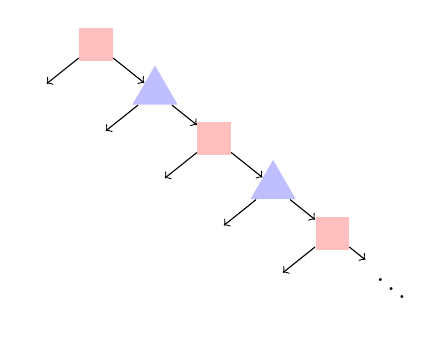
\begin{tikzpicture}
\tikzstyle{square}=[fill=red!25,minimum size=12pt]
\tikzstyle{triangle}=[regular polygon,regular polygon sides=3, fill=blue!25,minimum size=12pt]
\tikzstyle{leaf}=[circle, draw=black,double,inner sep=2pt]
\node[square] (N1) {} [->]
            child [level distance=0.6cm] {
                node {}
            }
            child [level distance=0.6cm] {
              node[triangle]  {}
              child {
                node {}
              }
              child  {
                node[square] { }
                child {
                  node {}
                }
                child {
                  node[triangle] {}
                  child {
                    node {}
                  }
                  child  {
                    node[square] (N7) { }
                    child {
                      node {}
                    }
                    child {
                      node {$\ddots$}
                    }
                  }
                }
              }
            }
;
%\draw [dashed,->] (N7) .. controls +(right:2cm) and +(up:1cm).. (N1);
\end{tikzpicture}

  \caption{Infinite tree}
  \label{fig:inftree}
\end{figure}

\subsection{Tabulation}
On the basis of the process tree, the relationships between inputs and
outputs can be obtained by following all paths in the tree, from the
root to each leaf. The contractions found on the path down to this
leaf, are conditions on the input, that should hold for the program to
return the output stored in the node.

Tabulation is the process of walking the tree and for each leaf write
down the input and output, together with the associated conditions
that should be obeyed by the input, to obtain the output.

As the process tree can be infinite, this table of input-output pairs
can be infinite as well.

\subsection{Inversion}
The final step of URA is to extract the answers for a given output
from the table of input-output pairs, to obtain the set of
corresponding input values. The desired output given as argument to
URA is unified with each output class in the table. If unification
succeeds, the resulting substitution is then applied to the relevant
input-specification and the set of contractions is checked for
contradictions.

\subsection{Perfect Process Trees}
A \textit{perfect} process tree \cite{gluck1993occam}, is a process
tree without any infeasible paths. A path is infeasible if there is no
input such that the path is taken. The universal solving algorithm
always constructs perfect process trees, as branches are only created
in the tree if no contradictions between contractions occur along the
path from the root and splits in the tree are \textit{perfect
  splits}. Splits are perfect as long as an input value only gives
rise to a single path through the tree. We will show how to obtain a
finite representation of a process tree, but in doing so, we will
discard perfectness of the process tree (still using perfect
splits). Infeasible walks can occur. In general, if a process tree
storing negative information is perfect, it can not be finite. This
will be detailed in Section \ref{sec:closed-ura}.

\section{Supercompilation}
\label{sec:supercompilation}
\begin{figure}
  \centering
  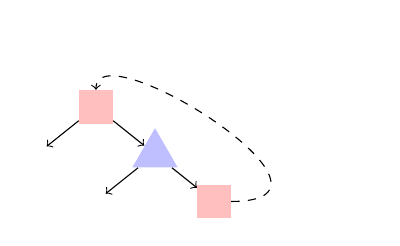
\begin{tikzpicture}
\tikzstyle{square}=[fill=red!25,minimum size=12pt]
\tikzstyle{triangle}=[regular polygon,regular polygon sides=3, fill=blue!25,minimum size=12pt]
\tikzstyle{leaf}=[circle, draw=black,double,inner sep=2pt]
\node[square] (N1) {} [->]
            child [level distance=0.6cm] {
                node {}
            }
            child [level distance=0.6cm] {
              node[triangle]  {}
              child {
                node {}
              }
              child  {
                node[square] (N7) { }
              }
            }
;
\draw [dashed,->] (N7) .. controls +(right:2cm) and +(up:1cm).. (N1);
\end{tikzpicture}
\caption{In supercompilation, back-edges are added from nodes that
  have ancestors of a common shape.}
  \label{fig:backedge}
\end{figure}

In supercompilation, one wishes to obtain more efficient programs by
observing their execution and generating new programs with equivalent
functionality. For instance two functions that operate independently,
might be more efficiently described by composing them into one program
(program composition). Another example is program specialization,
where parts of the input is known in advance, and supercompilation can
be a way of obtaining a more efficient version of the program when
this information is taken into account.

Supercompilation, like the universal resolving algorithm, makes a
controlled execution of the program, constructing a process tree of
the possible edges. In supercompilation, this technique of observing
the execution of a program is called \textit{driving}. The universal
resolving algorithm has been inspired by the techniques used in
supercompilation \cite{abramov2002principles}.

\subsection{Generalization}
In supercompilation the process trees are kept finite. Instead of
continuously \textit{driving} expressions, the driving steps are
interleaved with, with steps that decides whether a \textit{back edge}
can be made to a previous equivalent expression in an ancestor node.

This is still not enough to guarantee a finite tree, as there are
examples where the program iterates for ever, but continues to build
up larger and larger expressions, thus never finding a place to add a
back edge. This problem is solved by adding \textit{generalizing}
steps. Instead of checking that a \textit{renaming} of the expression
occurs as an ancestor, the ancestors are checked for another kind of
``similarity'' and if a similar ancestor is found, a generalised
expression of the node and the ancestor is made, such that they both
are instances of the new general node.

\section{Subject Language}
\label{sec:trfl}
In this paper we will study a small syntactically typed functional
language, that draws inspiration from both the language studied in
\cite{sorensen1998introduction} and the S-Graph language as defined in
the papers on the Universal Resolving Algorithm
\cite{abramov2000universal, abramov2002universal,
  abramov2002principles}.

\subsection{Syntax}
The syntax of our language is defined in Figure \ref{fig:bnf}. A
program, $p \in \mathcal{P}$, is a sequence of function definitions. A
function definition, $d \in \mathcal{D}$, can have two forms, either
they are pattern matching and are called \textit{G-functions} or they
are not and then called \textit{F-functions}. To distinguish, we use
the convention of naming all \textit{G-functions} with an initial
capital letter, and \textit{F-functions} with a lower case
letter. Functions can take any number of arguments and for
\textit{G-functions}, the first argument (and only that) must always
be a pattern-match.

Terms $t \in \mathcal{T}$ are either function calls (of the two
types), a conditional or an expression. We have two categories of
expressions. Atomic expressions, $ea \in \mathcal{A}$, can range over
only \textit{atoms} (which are prefixed with an apostrophe, such as
the symbol \texttt{'coffee}) and atomic variables $\texttt{.}x \in
\mathcal{A}$. This distinction between atomic variables
($\texttt{.}x$) and expression variables ($x$) serves as a simple type
system. A conditional can only compare atomic values and the only
comparison allowed is equality testing.

Ordinary expressions, can in addition to being atomic expressions, use
a \textit{cons}-operation to form pairs of values. These can be used
to construct lists, trees or other data-structures, as well as be used
for number-representation (Peano numerals).

\begin{figure}\centering
  \begin{align*}
    \mathcal{P} \ni p ::= & d^{+}\tag{Program}\\
    \mathcal{D} \ni d ::= &\texttt{fun \textit{\rmfamily fname} $x^{*}$ = $t$}  \tag{Definition} \\
    | \quad &\texttt{fun \textit{\rmfamily gname} [$x_1$, $x_2$] $x^{*}$ = $t_1$} \\
    & \texttt{\ \ | \textit{\rmfamily gname}\ \texttt{.}$x$ \hspace{.7cm} $x^{*}$ = $t_2$}\\
    \mathcal{T} \ni t ::= & \texttt{\textit{\rmfamily fname} $x^{*}$}  \tag{Term}\\
    | \quad & \texttt{\textit{\rmfamily gname} $x^{*}$} \\
    | \quad & \texttt{if $ea_1 = ea_2$ then $t_1$ else $t_2$} \\
    | \quad & e \\
    \mathcal{E} \ni e ::= & \texttt{[$e_1$, $e_2$]} \tag{Expression}\\
    | \quad & x \\
    | \quad & ea \\
    \mathcal{A} \ni ea ::= & \texttt{'}s \tag{Atomic expression}\\
    | \quad & \texttt{.}x
  \end{align*}
  \caption{Syntax of TRFL.}
\label{fig:bnf}
\end{figure}

As an example of how the syntax is used, the addition program
mentioned in the introduction is shown in Figure \ref{fig:addprog}.

\begin{figure}
  \centering
\begin{verbatim}
fun Add [s, ss] y = Add ss ['S, y]
  | Add .z y = if .z == 'Z then y
               else 'error-unknown-symbol
\end{verbatim}
  \caption{Addition in TRFL}
  \label{fig:addprog}
\end{figure}


\subsection{Value-classes}
Values in our language can either be \textit{atoms} or pairs of
values. Pairs are constructed using the \textit{cons}-operation as
described above. A value is \textit{ground} if it does not contain any
variables. We denote ground values as by $va \in AVal$ and $v \in Val$
depending on whether they only contain atoms.

\begin{figure}\centering
  \begin{align*}
    Val \ni v ::= & \texttt{[$v_1$, $v_2$]}\ |\ va\\
    AVal \ni va ::= & \texttt{'}s
  \end{align*}
  \caption{Values in TRFL.}
\label{fig:vbnf}
\end{figure}

As explained, the result of inverse-computation of non-injective
functions might result in several input values for one output. The set
of inputs might even be infinite. We represent these classes of
inputs, by placing meta-variables in the places where they vary, and
registering constraints that should be obeyed by these variables.  We
call such generalized values for \textit{C-expressions}, and we use
the word \textit{contractions} to denote the constraints on
meta-variables occurring in C-expressions. The domain of
C-expressions is shown in Figure \ref{fig:cbnf} as
$\mathcal{\widehat{A}}$ and $\mathcal{\widehat{E}}$. In addition we
define terms containing such meta variables, these are denoted
$\widehat{t} \in \widehat{\mathcal{T}}$.

A good analogy for these input-classes is the ZF-notation for
describing mathematical sets, where we represent the left-hand side by
\textit{C-expressions} and the right-hand side is used to specify the
constraints on the meta-variables occurring in the
\textit{C-expression}. 

\begin{figure}\centering
  \begin{align*}
    \widehat{\mathcal{T}} \ni \widehat{t}
      ::=& \texttt{\textit{\rmfamily fname} $x^{*}$} \tag{C-Term} \\
    | \quad & \texttt{\textit{\rmfamily gname} $x^{*}$} \\
    | \quad & \texttt{if $\widehat{ea_1} = \widehat{ea_2}$ then $\widehat{t_1}$ else $\widehat{t_2}$} \\
    | \quad & \widehat{e} \\
    \widehat{\mathcal{E}} \ni \widehat{e} ::=& \texttt{[$\widehat{e_1}$, $\widehat{e_2}$]} \tag{C-Expression} \\
    | \quad & \widehat{Xe} \\
    | \quad & \widehat{ea} \\
    \widehat{\mathcal{A}} \ni \widehat{ea} ::= & \texttt{'}s \tag{Atomic C-expression} \\
    | \quad & \widehat{Xa} \\
    \widehat{\mathcal{X}} \ni \widehat{x} ::= & \widehat{Xe} \tag{C-variable} \\
    | \quad & \widehat{Xa} \\
    \tag{Generalized C-term} \\
    \widehat{\mathcal{L}} \ni \widehat{l} ::= & \texttt{let $\widehat{x_1} = \widehat{e_1}$; $...$; $\widehat{x_n} = \widehat{e_n}$ in $\widehat{t}$} \\
    & \quad \textrm{where}\ n \in \mathbb{N}
  \end{align*}

\caption{Syntax of terms and expressions with meta variables}
\label{fig:cbnf}
\end{figure}

\subsection{Semantics}
Terms in TRFL are parameterized over an environment $\sigma$ and the
set of function definitions $\Gamma$. The operational semantics is
shown in Appendix \ref{sec:semantics}, Figure \ref{fig:semantics}
using judgement form: $\sigma |-_\Gamma t => (t', \sigma')$. A
judgement of this form should be interpreted as: \textit{given
  environment $\sigma$ and function definitions $\Gamma$, the term $t$
  steps to the term $t'$ and environment $\sigma'$.}

\section{Closed URA}
\label{sec:closed-ura}
Given a TRFL program and a partially specified input, the \emph{Closed
  URA} (CURA) algorithm first creates a process tree representing the
possible state transitions of the program, and then uses this tree to
search for possible inputs using a given output value. Like URA, the
tracing algorithm of CURA non-deterministically branches when it
cannot decide the flow of control resulting from the partially
specified input, applying \emph{perfect splits} to split the set of
possible inputs into disjoint sets, one for each branch.

As described earlier, URA is based on walking an often infinite
process tree, creating a table of pairs of output and input
sets. Because the process tree can be infinite, tracing of the process
tree has to be done on-line while tabulating input/output pairs. The
tracing step in CURA is an off-line algorithm that outputs a closed
representation of the process tree. The closed process tree is not a
solution to the inversion problem in itself, but can be used for
tabulation in the same way as URA, or it can be used to perform a
non-deterministic backwards search for input classes, given an output
value.

\subsection{Preliminaries}
We use the same definition of trees as in
\cite{sorensen1998introduction}. That is, a tree over a set $E$ is a
partial function $t : \mathbb{N}_1^\star \rightarrow E$, with the
usual restrictions required for representing finitely branching trees
(see \cite{sorensen1998introduction}\cite{courcelle1983fundamental}
for details).

By $\dom(t)$ we denote the set of nodes in tree $t$, and by
$t(\alpha)$ we denote the label at node $\alpha$. ${\rm anc}(t,
\alpha)$ denotes the set of ancestors for node $\alpha$ in tree
$t$. By $\anc(t, \alpha)$ we denote the set of nodes that are
ancestors to $\alpha$ in $t$, and for some $\alpha \in \dom(t)$,
$t\{\alpha \mapsto t'\}$ denotes the tree obtained from $t$ by replacing
the subtree rooted at node $\alpha$ with $t'$.

The tree $e \rightarrow e_1, ..., e_n$ is the tree with root labeled
$e$ and children labeled $e_1, ..., e_n$.

\subsection{Building the process tree}
The trace semantics for TRFL can be seen in Figure
\ref{fig:tracing}. We use the notation $X^\diamond$ for a fresh meta
variable. The semantics are non-deterministic when a branch cannot be
decided, and therefore describes an infinite process tree.

A C-term $\widehat{t}$ in our language fully describes a given set of
program states. The \textsc{If-*}, \textsc{Case-*} and \textsc{Call}
rules describe transitions between C-terms. Each transition is
associated with a \emph{contraction} $\kappa$, which reflects the
constraint that must be satisfied for the program input to reach the
given destination state. When multiple branches can be taken, the
contractions are guaranteed to split the input class into disjoint
sets. See Figure \ref{fig:edge} for the syntax of contractions.

For simplicity of the tracing rules, our trace semantics does not cut
\emph{infeasible branches}. However, as stated in
\cite{abramov2000universal}, even though the efficiency of the
algorithm may suffer, soundness and completeness is still preserved as
long as the tracing algorithm applies perfect splits along branches.

A let-term $\widehat{l}$ is used when we need to generalize a C-term
in order to ensure termination of the tracing algorithm. Transitions
for let-terms are described by the \textsc{Let-*} rules. A transition
between let-terms is associated with either a contraction $\kappa$ or
an \emph{expansion} $\sigma$.

A process tree is a tree $t$ with labels over $\Omega \times
\widehat{\mathcal{L}}$. For brevity, we write $t_\mathcal{L}(\alpha)$
for the $\widehat{\mathcal{L}}$-part of $t(\alpha)$ and
$t_\Omega(\alpha)$ for the $\Omega$-part. When building the process
tree for a given program, we start with the tree $(\kappa_{id},
\texttt{let $\emptyset$ in $\widehat{t_0}$}) \rightarrow$ consisting
of a single node with the initial program state $\widehat{t_0}$ as
label. Using the trace semantics, we iteratively add child nodes,
creating branches when multiple rules apply at the same time. For a
tree $t$ and a leaf node $\alpha \in \dom(t)$, we write ${\rm
  drive}(t, \alpha)$ to denote the tree obtained by exhaustively
applying the tracing rules on $t_\mathcal{L}(\alpha)$, adding the
resulting $\Omega \times \widehat{L}$ pairs as child nodes to
$\alpha$.

\begin{figure}
  \begin{align*}
    \mathcal{K} \ni \kappa ::= & \widehat{ea_1}~\#~\widehat{ea_2} \tag{Contraction} \\
                       | \quad & (\widehat{x} \mapsto \widehat{e})^{+} \\
    \Sigma \ni \sigma ::= & (\widehat{x} \gen \widehat{e})^{+} \tag{Expansion} \\
    \Omega \ni \omega ::= & \kappa ~|~ \sigma \tag{Edge label}
  \end{align*}
  \caption{Edge labels}
  \label{fig:edge}
\end{figure}

\begin{figure*}
  \begin{align}
    \nfrac{
      \widehat{ea_1} = \widehat{ea_2}
    }{
      |-_\Gamma \texttt{if $\widehat{ea_1}$ = $\widehat{ea_2}$ then $\widehat{t_1}$ else $\widehat{t_2}$} => <<\kappa_{id},\widehat{t_1}>>
    } \tagsc{If-Eq}
\\\nonumber\\
    \nfrac{
      \widehat{ea_1} \neq \widehat{ea_2} \quad \kappa = (\widehat{ea_1}\ \#\ \widehat{ea_2})
    }{
      |-_\Gamma \texttt{if $\widehat{ea_1}$ = $\widehat{ea_2}$ then $\widehat{t_1}$ else $\widehat{t_2}$} => <<\kappa, \widehat{t_2}>>
    } \tagsc{If-Neq-False}
\\\nonumber\\
    \nfrac{
      \widehat{ea_1} \neq \widehat{ea_2} \quad (\widehat{ea_1}\ \#\ \widehat{ea_2}) \not \in \textrm{Tauto} \quad \kappa = [\textrm{mkBind}(\widehat{ea_1}, \widehat{ea_2})]
    }{
      |-_\Gamma \texttt{if $\widehat{ea_1}$ = $\widehat{ea_2}$ then $\widehat{t_1}$ else $\widehat{t_2}$} => <<\kappa, \widehat{t_1}>>
    } \tagsc{If-Neq-True}
  \end{align}

  ~\newline

  \begin{align}
    \nfrac{
      \begin{array}{c}
        \widehat{e_0} = [\widehat{e_\alpha}, \widehat{e_\beta}] \quad \theta = \{ x_\alpha := \widehat{e_\alpha}, x_\beta := \widehat{e_\beta}, x_1 := \widehat{e_1}, ..., x_n := \widehat{e_n} \} \\
        \Gamma(\textit{gname}) =
        \begin{array}{l}
          \texttt{fun \textit{\rmfamily gname} [$x_\alpha$, $x_\beta$] $x_1$ $\ldots$ $x_n$ = $t_1$} \\
          \texttt{\ \ | \textit{\rmfamily gname}\ \texttt{.}$x$ \hspace{0.95cm} $x_1'$ $\ldots$ $x_n'$ = $t_2$} \\
        \end{array}
      \end{array}
    }{
      |-_\Gamma \texttt{\textit{\rmfamily gname} $\widehat{e_0}$ ... $\widehat{e_n}$} => <<\kappa_{id},  t_1 / \theta>>
    } \tagsc{Case-Cons}
\\\nonumber\\
    \nfrac{
      \begin{array}{c}
        \widehat{e_0} = \widehat{ea} \quad \theta = \{ .x := \widehat{ea}, x_1' := \widehat{e_1}, ..., x_n' := \widehat{e_n} \} \\
        \Gamma(\textit{gname}) =
        \begin{array}{l}
          \texttt{fun \textit{\rmfamily gname} [$x_\alpha$, $x_\beta$] $x_1$ $\ldots$ $x_n$ = $t_1$} \\
          \texttt{\ \ | \textit{\rmfamily gname}\ \texttt{.}$x$ \hspace{0.95cm} $x_1'$ $\ldots$ $x_n'$ = $t_2$} \\
        \end{array}
      \end{array}
    }{
      |-_\Gamma \texttt{\textit{\rmfamily gname} $\widehat{e_0}$ ... $\widehat{e_n}$} => << \kappa_{id}, t_2 / \theta>>
    } \tagsc{Case-Atom}
\\\nonumber\\
    \nfrac{
      \begin{array}{c}
        \widehat{e_0} = \widehat{Xe} \quad \theta = \{ x_\alpha := \widehat{X_{e_1}^\diamond}, x_\beta := \widehat{X_{e_2}^\diamond}, x_1 := \widehat{e_1}, ..., x_n := \widehat{e_n} \} \\
        \kappa = [\widehat{Xe} \mapsto [\widehat{X_{e_1}^\diamond}, \widehat{X_{e_2}^\diamond}]] \\
        \Gamma(\textit{gname}) =
        \begin{array}{l}
          \texttt{fun \textit{\rmfamily gname} [$x_\alpha$, $x_\beta$] $x_1$ $\ldots$ $x_n$ = $t_1$} \\
          \texttt{\ \ | \textit{\rmfamily gname}\ \texttt{.}$x$ \hspace{0.95cm} $x_1'$ $\ldots$ $x_n'$ = $t_2$} \\
        \end{array}
      \end{array}
    }{
      |-_\Gamma \texttt{\textit{\rmfamily gname} $\widehat{e_0}$ ... $\widehat{e_n}$} => <<t_1 / \theta, \kappa>>
    } \tagsc{Case-Var-Cons}
\\\nonumber\\
    \nfrac{
      \begin{array}{c}
        \widehat{e_0} = \widehat{Xe} \quad \theta = \{ .x := \widehat{X_{a}^\diamond}, x_1' := \widehat{e_1'}, ..., x_n' := \widehat{e_n'} \} \\
        \kappa = [\widehat{Xe} \mapsto \widehat{Xa^\diamond}] \\
        \Gamma(\textit{gname}) =
        \begin{array}{l}
          \texttt{fun \textit{\rmfamily gname} [$x_\alpha$, $x_\beta$] $x_1$ $\ldots$ $x_n$ = $t_1$} \\
          \texttt{\ \ | \textit{\rmfamily gname}\ \texttt{.}$x$ \hspace{0.95cm} $x_1'$ $\ldots$ $x_n'$ = $t_2$} \\
        \end{array}
      \end{array}
    }{
      |-_\Gamma \texttt{\textit{\rmfamily gname} $\widehat{e_0}$ ... $\widehat{e_n}$} => <<\kappa, t_2 / \theta>>
    } \tagsc{Case-Var-Atom}
  \end{align}

  ~\newline

  \begin{equation}
    \nfrac{
      \begin{array}{c}
        \Gamma(\textit{fname}) =
          \texttt{fun \textit{\rmfamily fname} $x_1$ $\ldots$ $x_n$ = $t$} \\
        \theta = \{ x_1 := \widehat{e_1}, ..., x_n := \widehat{e_n} \}
      \end{array}
    }{
      |-_\Gamma \texttt{\textit{\rmfamily fname} $\widehat{e_1}$ ... $\widehat{e_n}$} => << \kappa_{id}, t / \theta>>
    } \tagsc{Call}
  \end{equation}

  ~\newline

  \begin{align}
    \nfrac{
      L=\emptyset \quad |-_\Gamma \widehat{t} => << \kappa, \widehat{t'} >>
    }{
      |-_\Gamma \texttt{let $L$ in $\widehat{t}$} \rightharpoonup <<\kappa, \texttt{let $L$ in $\widehat{t'}$}>>
    } \tagsc{Let-NonProper}
\\\nonumber\\
    \nfrac{
     L = \texttt{$\widehat{x_1}$ = $\widehat{e_1}$; $...$; $\widehat{x_n}$ = $\widehat{e_n}$}\quad
     \omega = \{ \widehat{x_1} \gen \widehat{e_1}, ..., \widehat{x_n} \gen \widehat{e_n} \}
    }{
      |-_\Gamma \texttt{let $L$ in $\widehat{t}$} \rightharpoonup <<\omega, \texttt{let $\emptyset$ in $\widehat{t'}$} >>
    } (n > 0) \tagsc{Let-Proper}
  \end{align}

  \caption{Trace semantics}
  \label{fig:tracing}
\end{figure*}


\subsection{Closed process trees}
\label{sec:closed_tree}
Iteratively driving the leaves of a process tree until there are no
more leaf nodes for which the trace rules apply will not guarantee
termination of the tracing algorithm. In order to ensure termination,
we must employ some kind of stop criterion to prevent our algorithm
from going on indefinitely, while still ensuring that all possible
control flows are represented in the process tree.
\begin{definition}
  For some tree $t$ and leaf node $\alpha \in \dom(t)$, we say that
  $\alpha$ is \emph{processed} if $t_\mathcal{L}(\alpha)$ is not
  proper and at least one of the following is true:
  \begin{enumerate}
    \item $t_\mathcal{L}(\alpha) = \widehat{e}$ ~~ ($\alpha$ is a terminal node), or
    \item There exists some $\beta \in \anc(t, \alpha)$ such that
      $t_\mathcal{L}(\alpha)$ is a renaming of $t_\mathcal{L}(\beta)$,
      with preservation of variable types.
  \end{enumerate}
\end{definition}
If a node is processed, the algorithm will stop driving and proceed to
processing other leaf nodes until all nodes are processed.

The above stop criterion is sound with regards to ensuring that the
resulting process tree covers all possible control flows of the
program. Since we define renaming up to preservation of variable
types, and because we do not propagate negative information, driving
two nodes $\alpha, \beta \in \dom(t)$ where $t_\mathcal{L}(\alpha)$ is
a renaming of $t_\mathcal{L}(\beta)$ and $\alpha$ is a descendent of
$\beta$, will yield isomorphic process trees, up to renaming of
variables.

Using the above stop criterion alone will not ensure that the tracing
algorithm terminates in all cases, since it will fail to stop on
infinitely increasing terms. To accomodate for this, we introduce
\emph{abstractions}. In our definition of abstractions, we use the
notion of \emph{most specific generalizations} as defined in
\cite{sorensen1998introduction}:
\begin{definition}
  For some $\widehat{t_1},\widehat{t_2} \in \widehat{\mathcal{T}}$, we
  define the following:
  \begin{enumerate}
  \item We say that $\widehat{t_1} <<= \widehat{t_2}$ if there exists
    some substitution $\theta$ such that $\widehat{t_2} =
    \widehat{t_1}/\theta$.
  \item A term $\widehat{t_g}$ is a \emph{generalization} of
    $\widehat{t_1},\widehat{t_2}$ if $\widehat{t_g} <<= \widehat{t_1}$
    and $\widehat{t_g} <<= \widehat{t_2}$.
  \item A \emph{most specific generalization} of $\widehat{t_1},
    \widehat{t_2}$ is a generalization $\widehat{t_g}$ such that for
    every generalization $\widehat{t_g'}$, we have $\widehat{t_g'} <<=
    \widehat{t_g}$. We denote this by $\widehat{t_g} = \widehat{t_1}
    \sqcap \widehat{t_2}$.
  \end{enumerate}
\end{definition}
An abstraction is defined as follows:
\begin{definition}
  For $\alpha, \beta \in \dom(t)$ with $\widehat{l_g} =
  t_\mathcal{L}(\alpha) \sqcap t_\mathcal{L}(\beta)$ and
  $t_\mathcal{L}(\alpha) = \widehat{l_g} \{ \widehat{x_1} \mapsto
  \widehat{e_1}, ..., \widehat{x_n} \mapsto \widehat{e_n} \}$, we
  define
\begin{align*}
{\rm abstract}(t,\alpha,\beta) = t \{ \alpha \mapsto (t_\Omega(\alpha), \widehat{l_\alpha'})\rightarrow \}
\end{align*}
where
\begin{align*}
\widehat{l_\alpha'} = \texttt{let $\widehat{x_1}$ = $\widehat{e_1}$; $...$; $\widehat{x_n}$ = $\widehat{e_n}$ in $\widehat{l_g}$}
\end{align*}
\end{definition}

For example, if we have nodes $\alpha,\beta \in \dom(t)$ for some tree
$t$, with $t_\mathcal{L}(\alpha) = \texttt{let $\emptyset$ in $f
  ~\widehat{xs}$}$ and $t_\mathcal{L}(\beta) = \texttt{let $\emptyset$ in $f [a, as]$}$, with $\alpha$ being an ancestor of $\beta$, we are
not able to stop driving when reaching the node $\beta$, because
$t_\mathcal{L}(\beta)$ is larger than $t_\mathcal{L}(\alpha)$, and
therefore not a renaming. To solve this, we replace $t$ by $t' = {\rm
  abstract}(t, \beta, \alpha)$, which will replace $\beta$ with a node
with $\widehat{\mathcal{L}}$-label $\texttt{let $\widehat{xs}$ = $[a,
  as]$ in $f~\widehat{xs}$}$. This node can be driven using the
deterministic \textsc{Let-Proper} rule, resulting in a node with a
non-proper $\widehat{\mathcal{L}}$ label which is a renaming (with
$\theta = \emptyset$) of $t_\mathcal{L}(\alpha)$, and driving can
therefore be stopped.

Applying abstractions introduce \emph{expansions} in the process tree,
by the \textsc{Let-Proper} rule. An expansion specifies what
information was ``hidden'' by an abstraction, making it possible to
reconstruct this information when tabulating in a forward manner. When
doing a backwards search from a given output value, expansions are
used to tear down the structure of the output value when inferring the
possible input values.

\subsection{Criteria for generalization}
The ${\rm abstract}$ operation can be applied whenever a C-term is an
instance of some other C-term. Generalizing too often may be
undesirable, since it may lead to larger process trees, and it
therefore remains to specify \emph{when} to generalize.

In supercompilation\cite{sorensen1998introduction} this problem can be
solved using the \emph{homeomorphic embedding} relation $<|$, since
for any infinite sequence $\widehat{t_1}, \widehat{t_2}, ...$ of terms
over the same finite set of constructors, there is guaranteed to be
$\widehat{t_i} <| \widehat{t_j}$ for $i < j$\todo{reference
  courcelle}. The homeomorphic embedding relation on C-terms is the
smallest relation satisfying the rules defined in Figure
\ref{fig:embedding}.

\begin{figure*}\centering
  \begin{equation}
    \nfrac{
    }{
      \texttt{'}s_1 <| \texttt{'}s_2
    } (s_1 = s_2) \tagsc{Atoms}
  \end{equation}

  \begin{equation}
    \nfrac{
    }{
      \widehat{x_1} <| \widehat{x_2}
    }\tagsc{Variables}
  \end{equation}

  \begin{equation}
    \nfrac{
      \widehat{e_1} <| \widehat{e_1'}\quad \widehat{e_2} <| \widehat{e_2'}
    }{
      \texttt{[$\widehat{e_1}$, $\widehat{e_2}$]} <| \texttt{[$\widehat{e_1'}$, $\widehat{e_2'}$]}
    }
    \qquad
    \nfrac{
      \widehat{e} <| \widehat{e_1}
    }{
      \widehat{e} <| \texttt{[$\widehat{e_1}$, $\widehat{e_2}$]}
    }
    \qquad
    \nfrac{
      \widehat{e} <| \widehat{e_2}
    }{
      \widehat{e} <| \texttt{[$\widehat{e_1}$, $\widehat{e_2}$]}
    }
    \tagsc{Cons}
  \end{equation}

  \begin{equation}
    \nfrac{
      \widehat{ea_1} <| \widehat{ea_1'} \quad \widehat{ea_2} <| \widehat{ea_2'} \quad \widehat{t_1} <| \widehat{t_1'} \quad \widehat{t_2} <| \widehat{t_2'}
    }{
      \texttt{if $\widehat{ea_1}$ = $\widehat{ea_2}$ then $\widehat{t_1}$ else $\widehat{t_2}$} <| \texttt{if $\widehat{ea_1'}$ = $\widehat{ea_2'}$ then $\widehat{t_1'}$ else $\widehat{t_2'}$}
    } \tagsc{If-A}
  \end{equation}

  \begin{equation}
    \nfrac{
      \exists \widehat{t'} \in \{\widehat{ea_1}, \widehat{ea_2}, \widehat{t_1}, \widehat{t_2}\}. \widehat{t} <| \widehat{t'}
    }{
      \widehat{t} <| \texttt{if $\widehat{ea_1}$ = $\widehat{ea_2}$ then $\widehat{t_1}$ else $\widehat{t_2}$}
    } \tagsc{If-B}
  \end{equation}

\begin{equation}
  \nfrac{
    \forall i \in \{0, \ldots, n\}. \widehat{e_i} <| \widehat{e_i'}
  }{
    h(\widehat{e_0}, \ldots, \widehat{e_n}) <| h(\widehat{e_0'}, \ldots, \widehat{e_n'})
  } (h \in G \cup F)
  \qquad
  \nfrac{
    \exists i \in \{0, \ldots, n\}. \widehat{e} <| \widehat{e_i'}
  }{
    \widehat{e} <| h(\widehat{e_0'}, \ldots, \widehat{e_n'})
  }
 \tagsc{Call}
\end{equation}

\caption{Homeomorphic embedding relation}
\label{fig:embedding}
\end{figure*}


\subsection{Tracing algorithm}
The final tracing algorithm can be seen below. We say that a tree $t$
is \emph{closed} when all leaves in $t$ are processed.
\begin{algorithmic}
  \STATE {\bf input} $[\widehat{e_1}, ..., \widehat{e_n}) \in \widehat{\mathcal{E}}^\star$
  \STATE $t\gets (\kappa_{id}, \texttt{let $\emptyset$ in $main~\widehat{e_1}~...~\widehat{e_n}$})\rightarrow$
  \WHILE{$t$ is not closed}
    \STATE $\beta\gets\text{an unprocessed leaf node in $t$}$
    \STATE $A\gets\{ \alpha\in\anc(t,\beta) ~|~ \alpha\text{ not proper}, t(\alpha) \not<| t(\beta)  \}$
    \IF{$A = \emptyset$}
      \STATE $\textrm{drive}(t,\beta)$
    \ELSE
      \STATE {\bf let }$\alpha \in A$
      \IF{$t_\mathcal{L}(\alpha) \gen t_\mathcal{L}(\beta)$}
       \STATE $t\gets {\rm abstract}(t,\beta,\alpha)$
      \ELSIF{$t_\mathcal{L}(\alpha) \leftrightarrow t_\mathcal{L}(\beta)$}
        \STATE $t\gets {\rm drive}(t,\beta)$
      \ELSE
        \STATE $t\gets {\rm abstract}(t,\alpha,\beta)$
      \ENDIF
    \ENDIF
  \ENDWHILE
\end{algorithmic}


\subsection{Forward interpretation}
The process tree constructed by the above algorithm can be seen as a
flow-graph description of the original program. We can define the
\textit{forward} semantics of this flow-graph language, as a state
machine with transition function $\delta : Q \times
\mathcal{P}(\omega) -> Q \times \mathcal{P}(\omega)$, where $Q
\subseteq \mathbb{N}^{*}_1$ is the set of nodes occurring in the
process tree. That is, $\delta$ is a function from states and a set of
edge-labels as well.  A state $q_0 \in Q$ is a designated start state
and a subset $F \subseteq U$ are terminal nodes. As the process tree
is finite, these sets are finite as well.

The program can then be executed by binding constructing an
environment $\sigma$ where the meta variables representing the input
are bound to concrete values, and then applying the transition
function continuously: $\delta^{*}(q_o, \sigma)$, until we reach a
state in $F$. 

There are three possible transition rules, depending on the edge
labels collected and the edge labels on edges exiting from the current
state. An edge with a label $X_e |-> X_a$ can be taken when
$\sigma(X_e) = va$, for some atom $va$. The new environment $\sigma'$
will then be contain the binding $X_a |-> va$. An edge with a label
$X_e |-> \texttt{[}Xe_1\texttt{,}Xe_2\texttt{]}$, will likewise be
taken when $\sigma(X_e) = \texttt{[}v_1\texttt{,}v_2\texttt{]}$, for
some values $v_1$ and $v_2$. The new environment $\sigma'$ should then
be extended bindings: $X_1 |-> v_1$ and $X_2 |-> v_2$. An edge with
label $Xa_1\ \#\ Xa_2$ can only be followed when $\sigma(Xa_1) \neq
\sigma(Xa_2)$. An edge with labels $Xe_1 \gen Xe_2, Xe_3 \gen Xe_4,
\ldots, Xe_{n-1} \gen Xe_n$ will always be followed and will give rise
to the new bindings: $Xe_1 |-> Xe_2, Xe_3 |-> Xe_4, \ldots, Xe_{n-1}
|-> Xe_n$.

As our splits are perfect, $\delta$ will be deterministic and no two
edges can be followed from the same state.

\subsection{Backward interpretation}
In the case of backward interpretation we have to reverse all the
edges in the state machine defined by the process tree. In addition,
we will make our definitions easier by adding a new node with edges
\textit{to} all terminal nodes. This will be the starting state of the
inverse interpretation.

Now, the transition function will then again be defined of the type
$\delta : Q \times \mathcal{P}(\omega) -> Q \times
\mathcal{P}(\omega)$. This time however, the function will be
non-deterministic, thus multiple paths will be taken in the
flow-graph.

\section{Examples}
\subsection{Addition}
When executing our Closed URA on the addition example in Section
\ref{sec:trfl}, Figure \ref{fig:addprog}, we obtain the process tree
on Figure \ref{fig:addtree}. The dashed edge is a back-edge introduced
after a generalization step (as explained in Section
\ref{sec:closed_tree} the edge is implicit in our representation
of trees).

This process tree can be seen as a flow-graph representation of the
\texttt{Add} program. We can plug in values in place of $X_{in}$ and
$Yf_{in}$ and follow the graph while applying contractions,
substitutions and expansions along the way. When we reach a terminal
node the program terminates with the value in stored in the node.

\subsubsection{Forward interpretation}
We will now go through the evaluation of \texttt{Add} when $X_{in} =
\texttt{['S, 'Z]}$ and $Y_{in} = \texttt{'Z}$. At the root node it is
determined whether $X_{in}$ is an atom or a cons. As it is a cons, we
follow the right branch, creating two new variables $Xe_1$ and $Xe_2$
representing the head and the tail of $X_{in}$. The next edge contains
two contractions, in this case they can be seen as value bindings,
setting the variable on the left-hand side to the value on the right
hand side. Now we have $X_{in} = \texttt{'Z}$ and $Y_{in} =
\texttt{['S, 'Z]}$. We return to the root and proceed down the left
branch, as the $X_{in}$ variable contains \texttt{'Z}, we follow the
right branch and return $Y_{in}$.

\begin{figure*}
  \centering

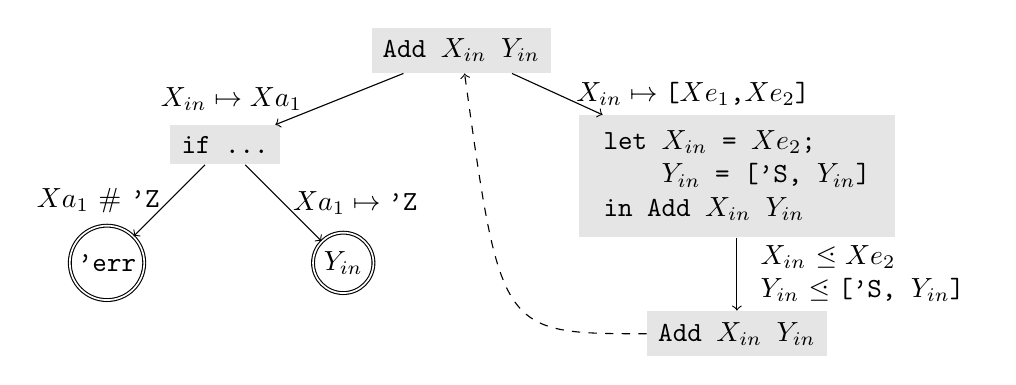
\begin{tikzpicture}
\tikzstyle{vtx}=[fill=black!10,minimum size=12pt,inner sep=4pt]
\tikzstyle{leaf}=[circle, draw=black,double,inner sep=2pt]
\node[vtx] (N2)  {\texttt{Add $X_{in}$ $Y_{in}$}} [->]
            child [sibling distance=6cm, level distance=1.2cm] {
                node[vtx] (N3)  {\texttt{if ...}}
                    child [sibling distance=3cm, level distance=1.5cm] {
                        node[leaf] (N4)  {\texttt{'err}}
                        edge from parent {
                          node[left] {$Xa_1\ \#\ \texttt{'Z}$}
                        }
                    }
                    child [sibling distance=3cm, level distance=1.5cm]{
                        node[leaf] (N5)  {$Y_{in}$}
                        edge from parent {
                          node[right] {$Xa_1 \mapsto \texttt{'Z}$}
                        }
                    }
                    edge from parent {
                      node[left] {$X_{in} \mapsto Xa_1\quad$}
                    }
            }
            child [sibling distance=7cm, level distance=1.6cm]{
                node[vtx] (N6)  {
                  $\begin{array}{l}
                    \texttt{let $X_{in}$ = $Xe_2$;} \\
                    \texttt{\ \ \ \ $Y_{in}$ = ['S, $Y_{in}$]} \\
                    \texttt{in Add $X_{in}$ $Y_{in}$}
                  \end{array}$
                }
                child [level distance=2cm] {
                  node[vtx] (N7) {
                    \texttt{Add $X_{in}$ $Y_{in}$}
                  }
                  edge from parent [left] {
                    node[right] {$
                      \begin{array}{l}
                        X_{in} \gen Xe_2 \\
                        Y_{in} \gen \texttt{['S, $Y_{in}$]}
                      \end{array}$}
                  }
                }
                edge from parent {
                  node[right] {\ $X_{in} \mapsto \texttt{[}Xe_1\texttt{,} Xe_2\texttt{]} \quad$}
                }
    }
;

\draw [dashed,->] (N7) .. controls +(left:3cm).. (N2);
\end{tikzpicture}
  \caption{Closed process tree for addition}
  \label{fig:addtree}
\end{figure*}


\subsubsection{Backward interpretation}
When executing the program backwards, we can start from any of the
terminal nodes. We unify the given output with all terminal nodes and
execute non-deterministically from all nodes that we can unify with.

Further explanation here ...


\begin{figure*}
  \centering

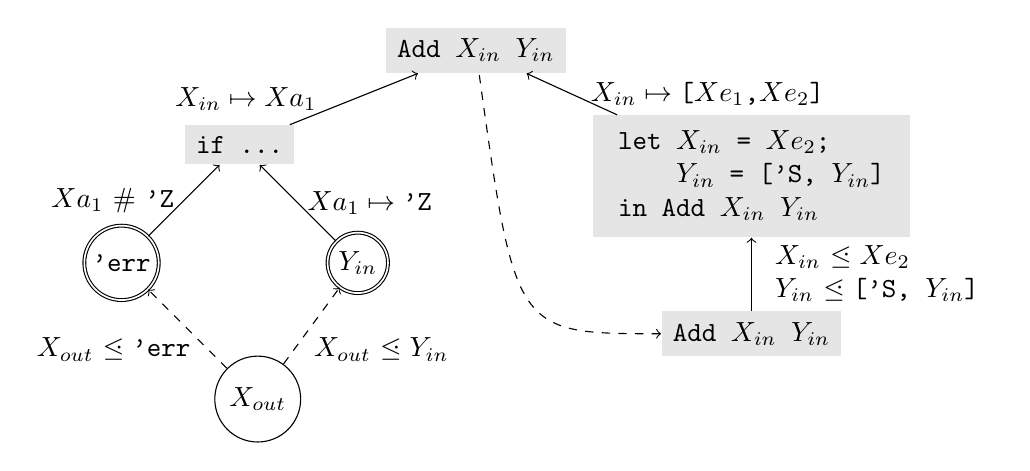
\begin{tikzpicture}
\tikzstyle{vtx}=[fill=black!10,minimum size=12pt,inner sep=4pt]
\tikzstyle{leaf}=[circle, draw=black,double,inner sep=2pt]
\node[vtx] (N2)  {\texttt{Add $X_{in}$ $Y_{in}$}} [<-]
            child [sibling distance=6cm, level distance=1.2cm] {
                node[vtx] (N3)  {\texttt{if ...}}
                    child [sibling distance=3cm, level distance=1.5cm] {
                        node[leaf] (N4)  {\texttt{'err}}
                        edge from parent {
                          node[left] {$Xa_1\ \#\ \texttt{'Z}$}
                        }
                    }
                    child [sibling distance=3cm, level distance=1.5cm]{
                        node[leaf] (N5)  {$Y_{in}$}
                        edge from parent {
                          node[right] {$Xa_1 \mapsto \texttt{'Z}$}
                        }
                    }
                    edge from parent {
                      node[left] {$X_{in} \mapsto Xa_1\quad$}
                    }
            }
            child [sibling distance=7cm, level distance=1.6cm]{
                node[vtx] (N6)  {
                  $\begin{array}{l}
                    \texttt{let $X_{in}$ = $Xe_2$;} \\
                    \texttt{\ \ \ \ $Y_{in}$ = ['S, $Y_{in}$]} \\
                    \texttt{in Add $X_{in}$ $Y_{in}$}
                  \end{array}$
                }
                child [level distance=2cm] {
                  node[vtx] (N7) {
                    \texttt{Add $X_{in}$ $Y_{in}$}
                  }
                  edge from parent [left] {
                    node[right] {$
                      \begin{array}{l}
                        X_{in} \gen Xe_2 \\
                        Y_{in} \gen \texttt{['S, $Y_{in}$]}
                      \end{array}$}
                  }
                }
                edge from parent {
                  node[right] {\ $X_{in} \mapsto \texttt{[}Xe_1\texttt{,} Xe_2\texttt{]} \quad$}
                }
    }
;

\node[circle,draw,below right=of N4] (END) {$X_{out}$};
\draw [dashed,->] (END) -- (N4);
\node at(-4.6,-3.8){$X_{out} \gen \texttt{'err}$};
\draw [dashed,->] (END) -- (N5);
\node at(-1.2,-3.8){$X_{out} \gen \texttt{$Y_{in}$}$};
\draw [dashed,<-] (N7) .. controls +(left:3cm).. (N2);
\end{tikzpicture}
\caption{Closed process tree for addition, with edges reversed and new
  combined starting state.}
  \label{fig:addtree}
\end{figure*}


\section{Future Work}
\subsection{Size-change termination analysis}
\todo{Rewrite this section}
  The Size-Change Termination Analysis (SCTA)\cite{lee2001size} can be
  used to identify programs that terminate for all inputs, and
  size-change graphs resulting from this approach may be used to cut
  branches in a process tree, minimizing its size. We are not aware of
  any uses of SCTA in the field of inverse interpretation, but in this
  report we will investigate whether this approach is feasible.



\bibliographystyle{abbrvnat}
\bibliography{../bibliography}


\appendix
\section{TRFL Semantics}
\label{sec:semantics}


\begin{minipage}{2\linewidth}
  \centering

  \begin{equation}
    \nfrac{
      ea_1/ \sigma = ea_2/\sigma \quad
    }{
      \sigma |-_\Gamma \texttt{if $ea_1$ = $ea_2$ then $t_1$ else $t_2$} => (t_1, \sigma)
    }
    \qquad
    \nfrac{
      ea_1/ \sigma \neq ea_2/\sigma \quad
    }{
      \sigma |-_\Gamma \texttt{if $ea_1$ = $ea_2$ then $t_1$ else $t_2$} => (t_2, \sigma)
    } \tagsc{If}
\end{equation}

\begin{equation}
\hspace{-0.7cm}
  \nfrac{
    \begin{array}{c}
      \Gamma(\textit{gname}) =
      \begin{array}{l}
        \texttt{fun \textit{\rmfamily gname} [$x_\alpha$, $x_\beta$] $x_1$ $\ldots$ $x_n$ = $t_1$} \\
        \texttt{\ \ | \textit{\rmfamily gname}\ \texttt{.}$x$ \hspace{1.1cm} $x_1'$ $\ldots$ $x_n'$ = $t_2$} \\
      \end{array} \\
      e_0/\sigma = \texttt{[$v_1$, $v_2$]} \\
      \sigma' = \sigma\{x_\alpha |-> v_1, x_\beta |-> v_2, x_1 |-> e_1/\sigma, \ldots, x_n |-> e_n/\sigma\} 
    \end{array}
  }{
    \sigma |-_\Gamma \texttt{\textit{\rmfamily gname} $e_0$ $e_1$ $\ldots$ $e_n$} => (t_1, \sigma')
  }
\qquad
  \nfrac{
    \begin{array}{c}
      \Gamma(\textit{gname}) =
      \begin{array}{l}
        \texttt{fun \textit{\rmfamily gname} [$x_\alpha$, $x_\beta$] $x_1$ $\ldots$ $x_n$ = $t_1$} \\
        \texttt{\ \ | \textit{\rmfamily gname}\ \texttt{.}$x$ \hspace{1.1cm} $x_1'$ $\ldots$ $x_n'$ = $t_2$} \\
      \end{array} \\
      \sigma' = \sigma\{\texttt{.}x |-> \texttt{'}s, x_1' |-> e_1/\sigma, \ldots, x_n' |-> e_n/\sigma\}
    \end{array}
  }{
    \sigma |-_\Gamma \texttt{\textit{\rmfamily gname} $e_0$ $e_1$ $\ldots$ $e_n$} => (t_2, \sigma')
  }
  \tagsc{Call-G}
\end{equation}

\begin{equation}
  \nfrac{
    \begin{array}{c}
      \Gamma(\textit{fname}) =
        \texttt{fun \textit{\rmfamily fname} $x_1$ $x_2$ $\ldots$ $x_n$ = $t$}
        \\
      \sigma' = \sigma\{x_1 |-> e_1/\sigma, x_2 |-> e_2/\sigma, \ldots, x_n |-> e_n/\sigma\} 
    \end{array}
  }{
    \sigma |-_\Gamma \texttt{\textit{\rmfamily fname} $e_1$ $e_2$ $\ldots$ $e_n$} => (t, \sigma')
  } \tagsc{Call-F}
\end{equation}

\figcaption{Operational Semantics for TRFL.}
\label{fig:semantics}
\end{minipage}



\begin{figure*}\centering



\end{figure*}





\end{document}
